\documentclass{article}
\usepackage{xparse}
\usepackage{graphicx}
\usepackage{float}

\title{SafeStreets}
\author{Marco Premi, Fabrizio Siciliano, Giuseppe Taddeo}
\pagestyle{headings}

\begin{document}
\maketitle

\tableofcontents

\newpage
\section{Introduction}
\subsection{Purpose}
\subsubsection{General Purpose}
    The purpose of this document is to correctly analyze all requirements, 
    goals and actions needed in order to correctly develop SafeStreets.\\
    \\
    SafeStreets is a crowd-sourced application that intends to provide users
    with the possibility to notify authorities when traffic violations occur
    (eg. traffic violations) and will help to maintain stability and order
    within the streets. A reporting system will also be available to police
    offices and municipality employees in order to allow them to analyze (and take
    actions accordingly) different areas of the city and assess which areas have
    the most violations committed in.\\
    \\
    The core application will focus on storing useful traffic violation data
    provided by users, mainly with the help of input forms and hard evidence
    such as images. At any violation input, SafeStreets will also store useful
    metadata such as date and time the violation was retrieved, geolocate where
    it is and update a city wide map highlighting the areas where violations
    happen.\\
    \\
    In addition to that, with the help of third parties (eg. municipality),
    SafeStreets will be able to retrieve the data given by such party and
    cross-reference them with its own data retrieved by users. By doing so, it
    will be possible to identify unsafe areas, assess which kind of problems
    happen more frequently and suggest possible intervention. It will also be
    possible for third parties (municipality and police officers) to
    automatically generate traffic tickets. This will be happening in order to
    cross-reference all available data in order to build statistics such as the
    most (or less) egregious offenders or the effectiveness of the SafeStreets
    initiative \subsubsection{Goals} Follows a list of all goals that will be
    reached with the SafeStreets initiative.
    \begin{itemize}
        \item G1: The system must allow all kind of users (both third parties
        and civilians) to correctly input (with hard evidence) traffic
        violations around the city;
        \item G2: The system must autonomously retrieve metadata from hard
        evidence useful to report and to all users;
        \item G3: The system must allow to create different clearance levels in
        order to offer different reporting systems to different kind of users;
        \item G4: The system will provide an efficient reporting system in order
        to highlight different violation categories through all parts of the
        city where the initiative is active;
    \end{itemize}
\subsection{Scope}
With SafeStreets users can notify the authorities when traffic violations occur,
and in particular parking violations. Both user and authorities must register to
the application and agree that SafeStreets stores the information provided,
completing it with suitable meta-data. The whole system, because it tracks users
information, must respect the standards defined for processing of sensitive
information such as GDPR if it is used in Europe. The user sends the type of the
violation to the municipality and direct proofs of it (like a photograph). The
system runs an algorithm to read the license plate and also asks the user to
directly insert the license for a better recognition. Of course other
information are required, like the name of the street when the violation has
occurred, which can be retrieved from user's direct input or from the
geographical position of the violation (using Google Maps API). Both users and
authorities can highlight the streets with the highest frequency of violations
or the vehicles that commit the most violations. SafeStreets crosses information
about the accidents that occur on the territory of the municipality with his own
data to identify potentially unsafe areas and suggest possible interventions.
Because municipality could generates traffic tickets from the information about
violations SafeStreets should guarantee that information is never altered (if a
manipulations occurs, the application should discard the information). Such
features are made possible trough the use of two mobile applications(one for the
citizens and one for the officers on the field). The collected information are
sent to a back-end. All the services can also be accessed through a specific
web-site. 
\subsection{Definitions, Acronyms, Abbreviations}
\subsubsection{Definitions}
\paragraph{User:} it is identified as a civilian customer of the product. It
will be the main source for the SafeStreets initiative to obtain information
about traffic violations and therefore be successful; \paragraph{Third
parties:}those kind of organization/company that could provide services useful
to SafeStreets and that will be able to retrieve data in order to improve the
streets' safety; \paragraph{Customer:} it defines both third party SafeStreets
users (police officers or municipality employees) and civilians; \paragraph{Ghiro:} image
manipulation detection software, used by third party users in order to detect
any image manipulation and assess the veracity of the hard evidence connected to
the traffic ticket
\subsubsection{Acronym}
\paragraph{UI:} User Interface \paragraph{GDPR:} General Data Protection
Regulation \paragraph{API:} Application Programming Interface \paragraph{GPS:}
Global Positioning System
\subsubsection{Abbreviations}
\paragraph{Gn:} nth goal; \paragraph{Dn:} nth domain; \paragraph{Rn:} nth
requirement;
\subsection{Revision History}
\subsection{Reference Documents}
\subsection{Document Structure}
\paragraph{Chapter 1 - Introduction}
Gives an introduction to the problem by describing the purpose of SafeStreets.
It also shows the goals and the scope of the application. 
\paragraph{Chapter 2 - Overall Description}[H]
Offers an overall description of the project. It identifies the actors involved
in the application and lists all the assumptions in order to identify all the
boundaries of the project. The product perspective includes details on the
shared phenomena and the domain models. The class diagram describe the domain
model used and the state diagrama analyzes:
\begin{itemize}
    \item The process of collecting violations from users
    \item The process of sharing informations with the municipality
\end{itemize}
The majority of functions of the system are more precisely specified by taking
in mind the goals of the system.  
\paragraph{Chapter 3 - Specific Requirements}
Contains external interface requirements which are: user interfaces, hardware
interfaces, software interfaces and communication interfaces. Few scenarios
describing how the system acts in real world are listed here. Furthermore it
provides the description of the functional requirements, through the use of use
cases and sequence diagrams. The non-functional requirements are defined through
performance requirements, design constraints and software system attributes.
\paragraph{Chapter 4 - Formal analysis using Alloy}
Includes the alloy model of some critical aspects with comments and
documentation.
\paragraph{Chapter 5 - Effort Spent}
Shows the effort spent by each single group member while working on the RASD.
\paragraph{Chapter 6 - References}
Includes the documents we used as reference.

\newpage
\section{Overall Description}
\subsection{Product Perspective}
SafeStreets is designed to be a completely new software applications. It uses
some already proven services (Google Maps, PlateRecognizer APIs and Ghiro
software) for its critical tasks. The software uses these services in order to
double check whether both addresses and license plates are correctly
standardized in order to be stored into the violations database and if the
collected hard evidence have been somehow manipulated or corrupted.\\
The system is composed of two different mobile applications: one for the
citizens that want to reports violations and one for the officers acting on the
field. It also provides a web site for third party users which allows them to
assess and analyze potential unsafe areas, thanks also to a powerful reporting
system.\\
Taken into consideration that the municipality could generate traffic tickets
from the input violations, the software will be critical when it comes to
handling chain of custody. The latter is assured to never be broken by not
allowing any kind of customer (user, PO or employee) to modify the reported violation. Supposedly, when
some traffic violations might be erroneous or do not have any reason of
existence, the inputting user can warn the responsible third party by attaching
a warning explaining why it should not be taken into consideration. The systems
also ensures the veracity of each violation and the hard evidence attached to it
by running a image manipulation detection software (Ghiro, per instance). This process is used by
third parties before the emission of each ticket to the corresponding offender.\\
\\
A high-level class diagram can be found below, which provides a model of the
application domain. The most important classes (not all of those which will be
implemented once the software will be ready) are shown in order to define how
the different components of SafeStreets will be communicating with each other.
It is possible to identify two kinds of third party users: police officers and
municipality employees. The first ones will be given access to both mobile
application and web application; the latter will be provided access just to the
above mentioned web application which will help these users assess the veracity of the hard
evidence attached to the traffic violations and to further analyze unsafe areas
around the municipality.\\

\begin{figure}[H]
    \centering
    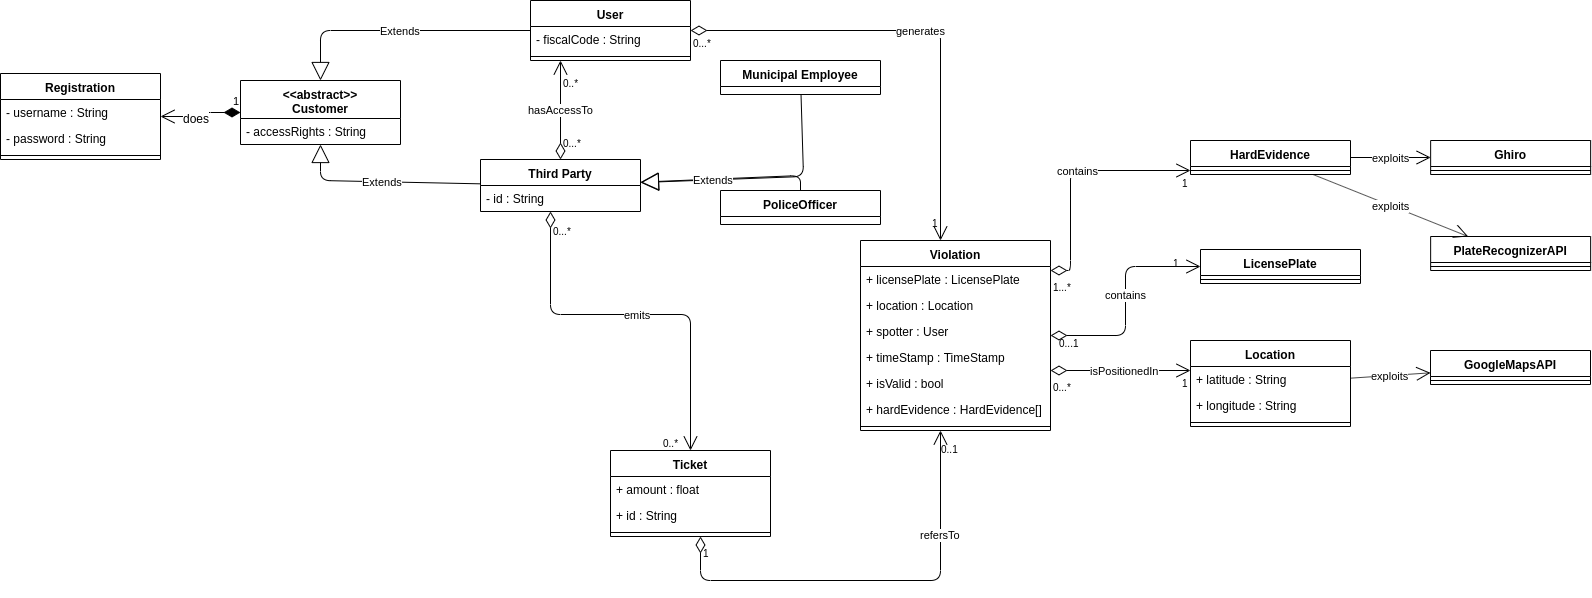
\includegraphics[scale=0.255]{Images/umlmodel}
    \caption{Class diagram}
\end{figure}

Each customer will be provided with a clearance level defined by a string 
\subsection{Product Functions}
In the following section the most important product functions of the system are reported.
%qua vanno aggiunte le varie funzioni
\subsection{User characteristics}
\subsection{Assumptions, dependencies and constraints}
\subsubsection{Assumptions}
\subsubsection{Dependencies}
\subsubsection{Constraints}

\newpage
\section{Specific Requirements}
\subsection{External Interface Requirements}
\subsubsection{User Interfaces}
\begin{figure}[H]
    \centering
    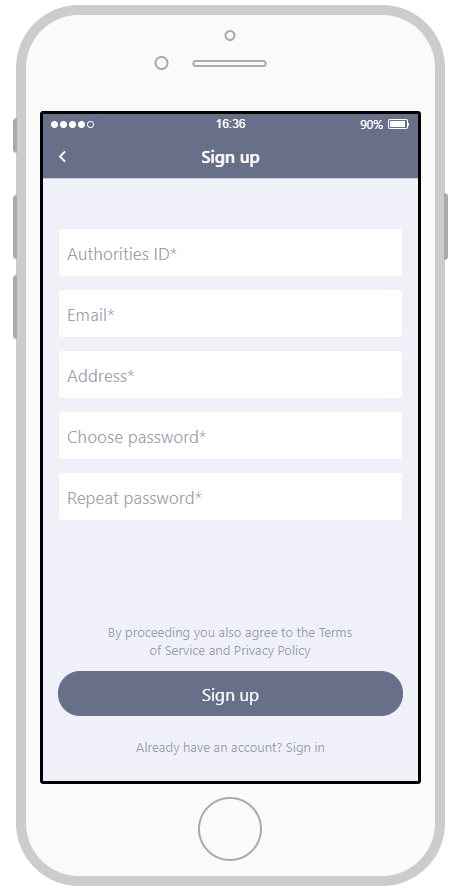
\includegraphics[scale=0.7]{Images/SignUpAuthoritiesApp}
    \caption{SignUp authorities}
\end{figure}
\begin{figure}[H]
    \centering
    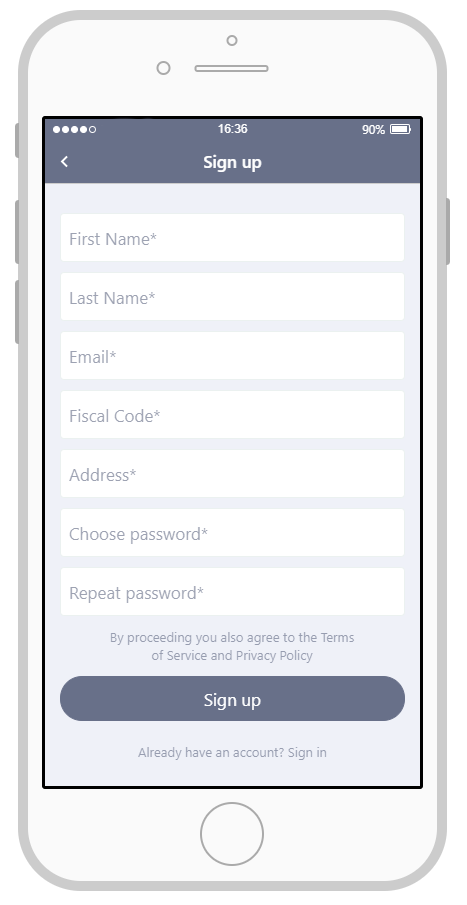
\includegraphics[scale=0.7]{Images/SignUpUtenteAPP}
    \caption{SignUp User}
\end{figure}
\begin{figure}[H]
    \centering
    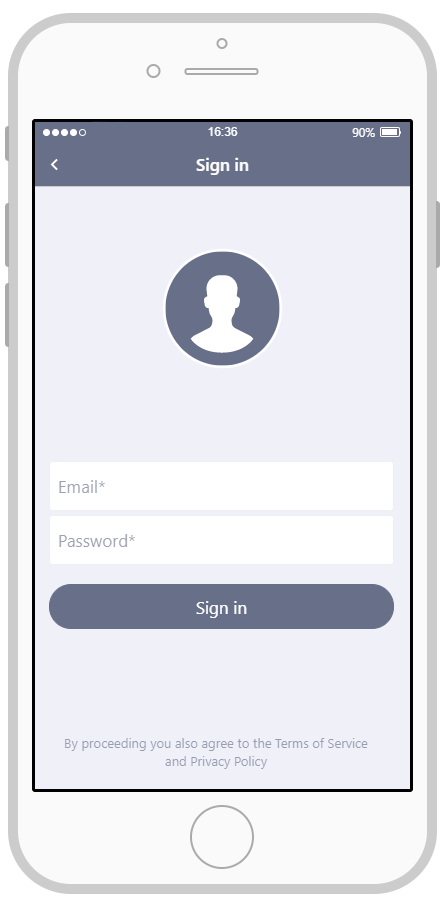
\includegraphics[scale=0.7]{Images/SignInAPP}
    \caption{SignIn}
\end{figure}
\begin{figure}[H]
    \centering
    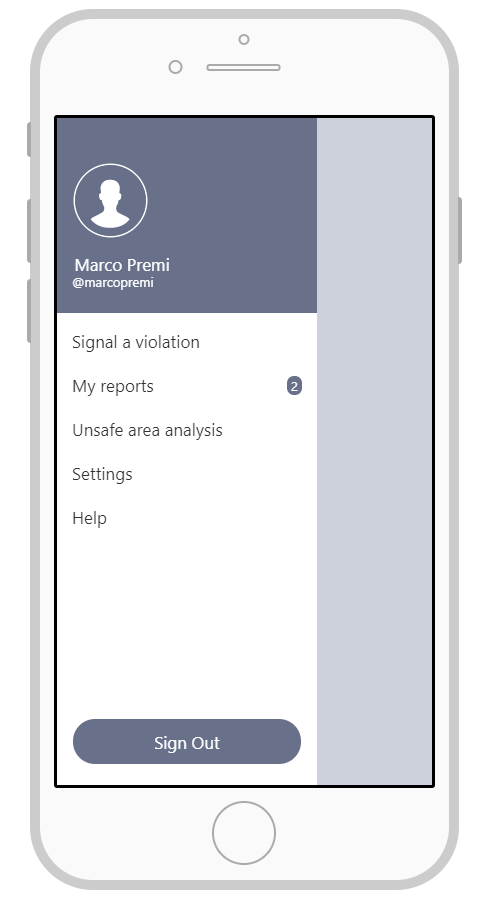
\includegraphics[scale=0.7]{Images/MenuAPP}
    \caption{Menu}
\end{figure}
\begin{figure}[H]
    \centering
    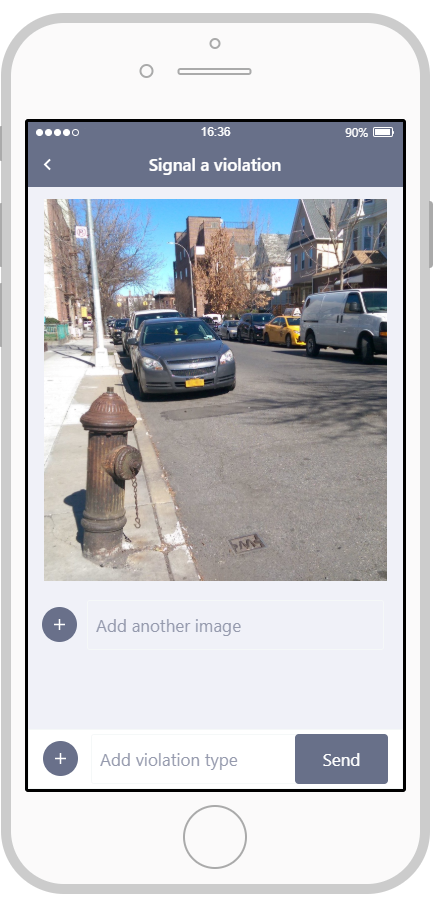
\includegraphics[scale=0.7]{Images/SignalAViolationAPP}
    \caption{SignIn}
\end{figure}
\begin{figure}[H]
    \centering
    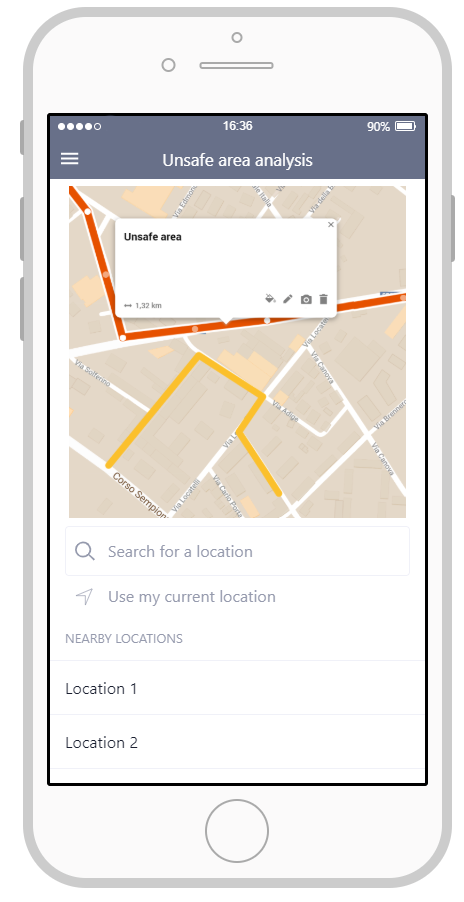
\includegraphics[scale=0.7]{Images/UnsafeAreaAnalysisAPP}
    \caption{SignIn}
\end{figure}
\begin{figure}[H]
    \centering
    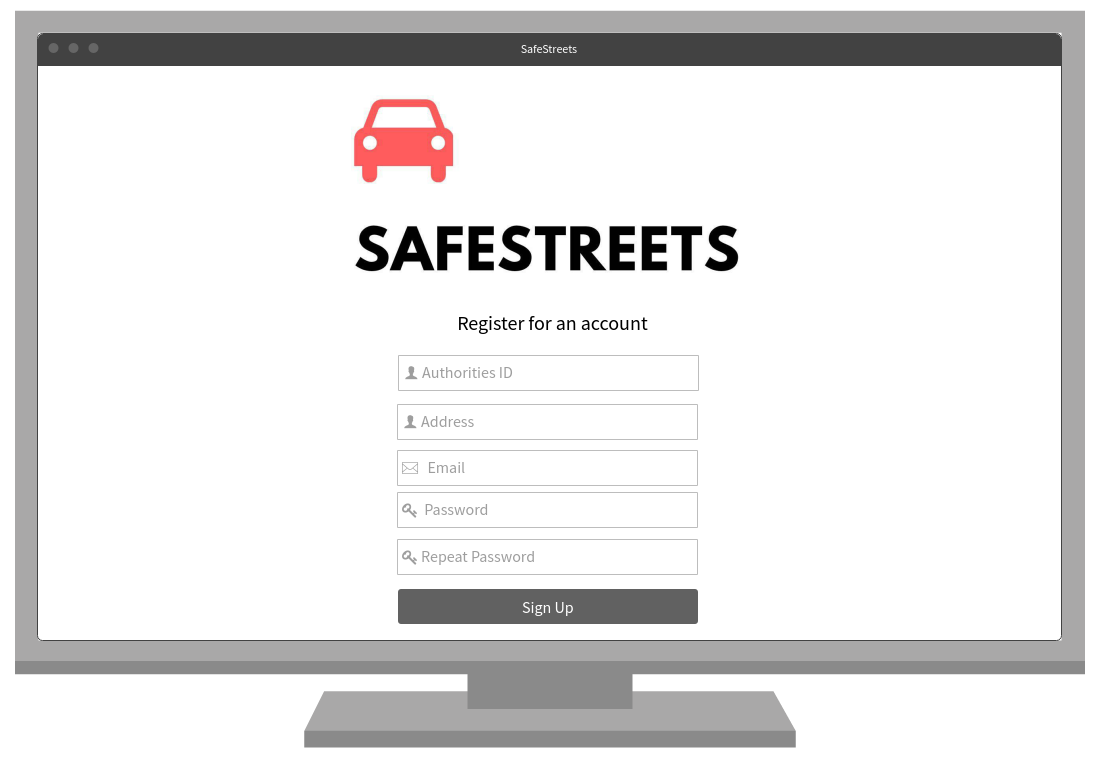
\includegraphics[scale=0.35]{Images/WEBSignUp}
    \caption{SignUp}
\end{figure}
\begin{figure}[H]
    \centering
    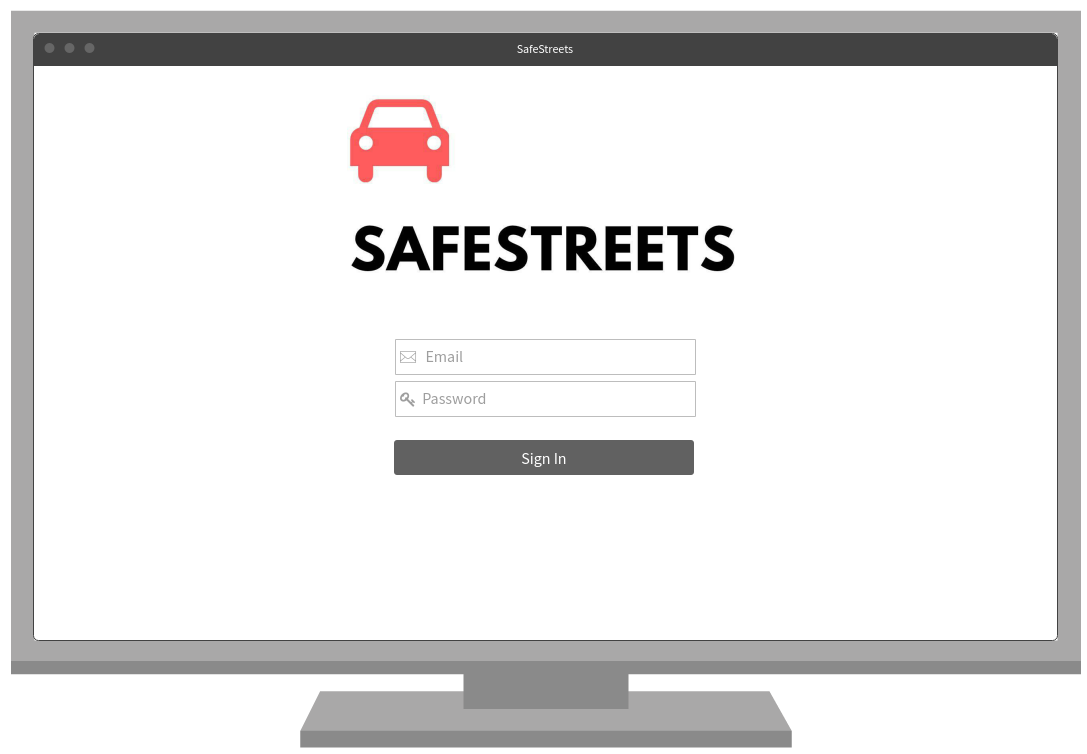
\includegraphics[scale=0.35]{Images/WEBSignIn}
    \caption{SignIn}
\end{figure}
\begin{figure}[H]
    \centering
    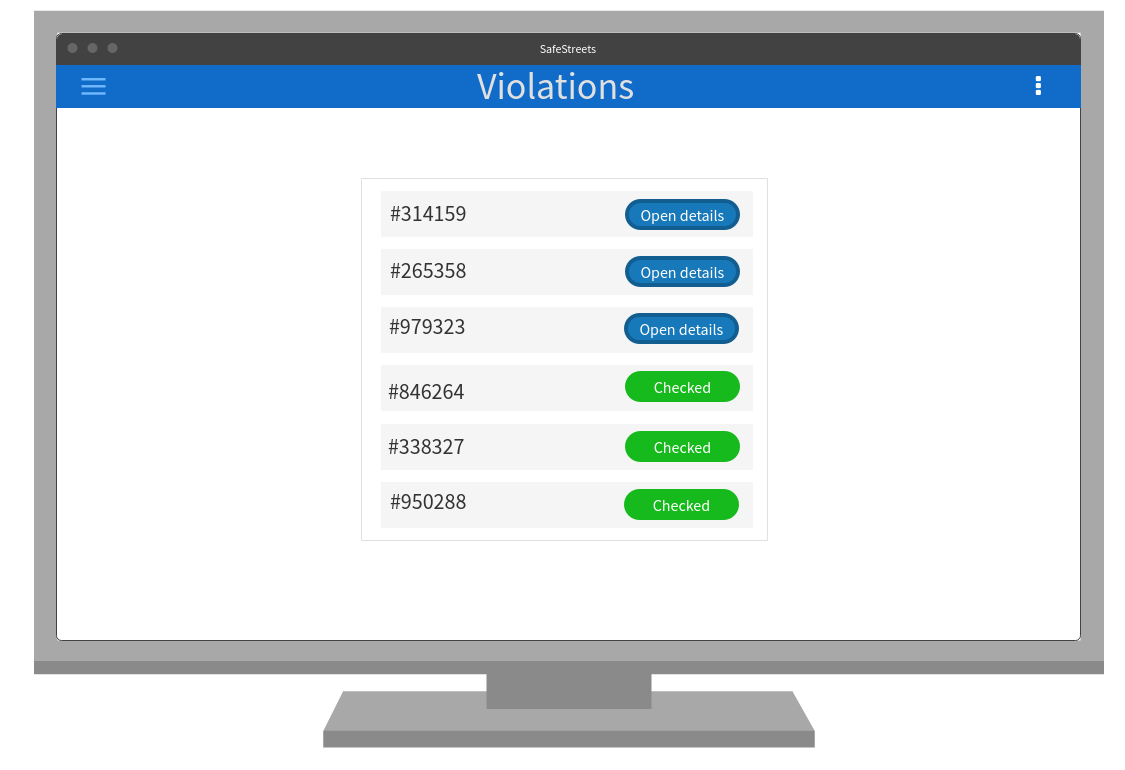
\includegraphics[scale=0.35]{Images/WEBViolations}
    \caption{Violations}
\end{figure}
\begin{figure}[H]
    \centering
    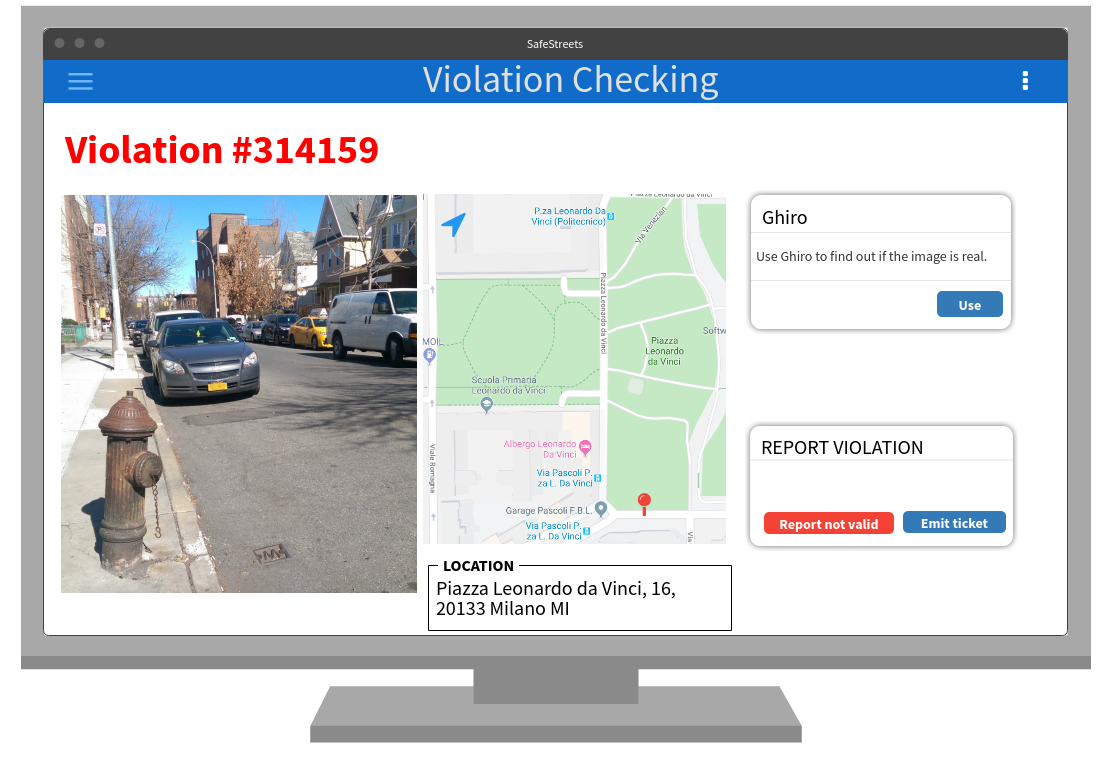
\includegraphics[scale=0.35]{Images/WEBViolationChecking}
    \caption{Violations checking}
\end{figure}
\begin{figure}[H]
    \centering
    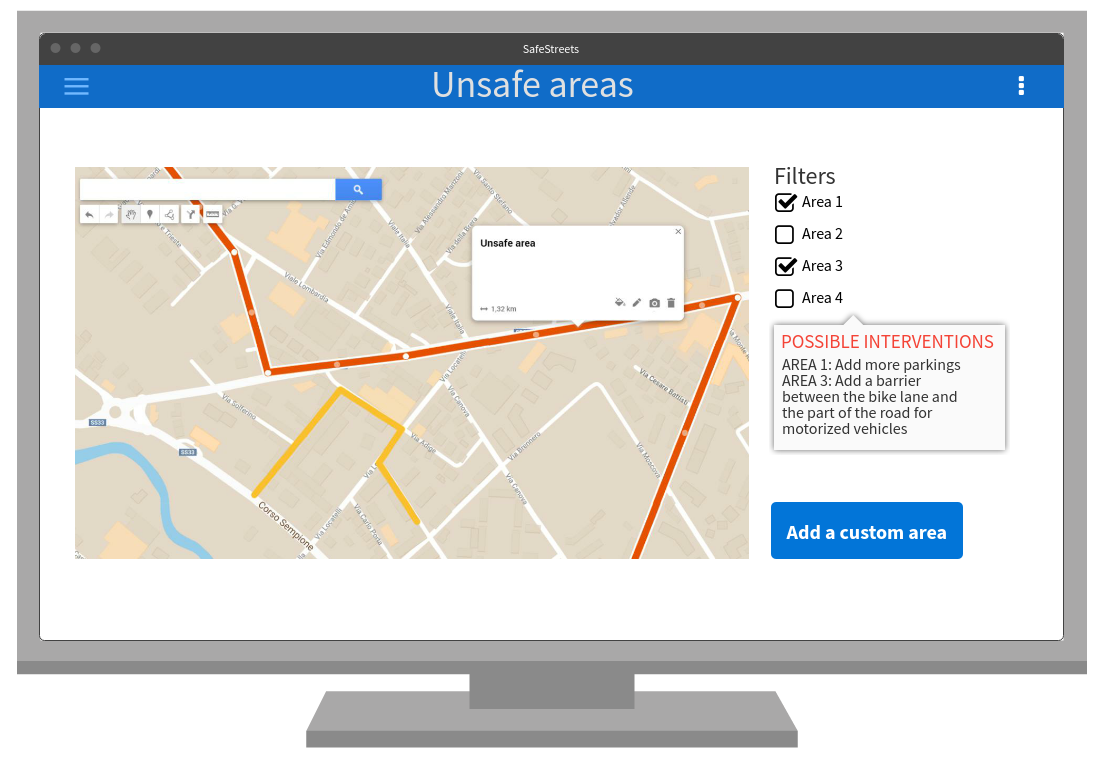
\includegraphics[scale=0.35]{Images/WEBUnsafeAreas}
    \caption{Unsafe Areas}
\end{figure}
\newpage
\newpage
\subsubsection{Hardware Interfaces}
The system has no hardware interfaces.
\subsubsection{Software Interfaces}
The system doesn't provide any API to external applications.\\
However some softwares part of SafeStreets is developed by other companies.
\begin{itemize}
    \item Google Maps API: for localization and creation of unsafe areas.
    \item Plate Recognizer API: for License Plate recognition.
    \item Ghiro: a digital image forensics tool used for find out if the image
    in the violation report is real.
\end{itemize}
\subsubsection{Communication Interfaces}
The system only uses HTTP(more precisely HTTPS) as communication service.
HTTP/HTTPS is used for:
\begin{itemize}
    \item User and third parties registration.
    \item Sending violations both to SafeStreets and to authorities.
    \item Using Google Maps API, Plate Recognizer API and Ghiro
\end{itemize}
\subsection{Scenarios}
\subsection{Functional requirements}
\subsection{Use Cases}
\subsubsection{User use cases}
\subsubsection{Third party use cases}

\subsection{Performance requirements}
\subsection{Design Constraints}
\subsubsection{Standars compliance}
With regard to the privacy, security for the mobile application and the back-end
is a big issue, so the whole project is subject to the the GDPR. Furthermore it's
a good practice to apply W3C's Standards to ensure intercompatibility.
\subsubsection{Hardware Limitations}
Even if SafeStreets is a software-based service there are some hardware
limitations regarding the smartphones.
\begin{itemize}
    \item must be able to make HTTPS requests (connection to internet 4G/3G/2G/Wi-Fi)
    \item must have on board GPS
\end{itemize}
\subsubsection{Any Other Constraint}
%probabilmente da cancellare
\subsection{Software System Attributes}
\subsubsection{Reliability}
\subsubsection{Availability}
\subsubsection{Security}
\subsubsection{Mantainability}
\subsubsection{Portability}

\newpage
\section{Formal Analysis using Alloy}

\newpage
\section{Effort spent}
\begin{center}
    \begin{tabular}{c|c|c|c|c}
        \hline
        \textbf{Description of the task} & \textbf{MP} & \textbf{FS} &
        \textbf{GT} \\
        Introduction                    & 2.5   & 2     & 0     \\
        Overall Description             & 1.5   & 3   & 0     \\
        Specific requirements           & 0     & 0     & 0     \\
        Formal analysis using Alloy     & 0     & 2     & 0     \\
    \end{tabular}
\end{center}
\section{References}
    \paragraph{Plate Recognizer:} https://app.platerecognizer.com
    
\end{document}  